\documentclass[aspectratio=169]{beamer}

\usepackage[UTF8, heading]{ctex} % 中文支持
\usepackage{color}
\usepackage{amsmath}
\usepackage{svg}          % 插入 svg 矢量图
\usepackage{tikz}         % 绘图
\usepackage{subcaption}   % 创建子图
\usepackage{minted}       % 代码高亮
\usepackage{algorithm2e}  % 伪代码
\usepackage{lmodern}      % 消除 warning
\usepackage{ncepu-beamer} % 应用主题

% 指定 inkscape 路径(inkscape 用于处理 svg 矢量图)
\setsvg{inkscapeexe={"C:/Program Files/Inkscape/bin/inkscape.com"}}
% 设置 svg 文字随图片缩放
\svgsetup{inkscapelatex=false}
% NOTE: draw.io 中的文本需要关闭自动换行和格式化文本

% 输入信息
\title{CostAware论文汇报}
\author{刘肇泽}
\institute{控制与计算机工程学院}
\date{\today}

\begin{document}

\begin{frame}[noframenumbering]

    \titlepage

\end{frame}

\begin{frame}{目录}

    \centering
    \begin{minipage}{0.8\textwidth}
        \tableofcontents
    \end{minipage}

\end{frame}

\section{问题背景}

\begin{frame}{云服务器任务调度模型}

    \begin{columns}
        \column{0.4\textwidth}

        任务调度流程:
        \begin{enumerate}
            \item 用户提交任务
            \item 任务调度器根据\textcolor{blue}{任务属性}和\textcolor{blue}{虚拟机状态}为任务分配虚拟机
        \end{enumerate}

        \column{0.6\textwidth}

        \begin{figure}
            \centering
            \includesvg[width=\textwidth]{pics/module.drawio.svg}
            \caption{云服务器任务调度模型}
        \end{figure}

    \end{columns}

\end{frame}


\section{数学模型}

\subsection{任务模型}

\begin{frame}{任务属性}

    对于用户提交的每个任务都具有如下属性:

    \begin{itemize}
        \item $ID$:任务编号
        \item $reqCom$:总计算量
        \item $T_{submit}$:提交时刻
        \item $QoS$:响应时间指标
        \item $Type$:任务类型
              \begin{itemize}
                  \item 计算敏感型
                  \item I/O敏感型
              \end{itemize}
    \end{itemize}
\end{frame}

\begin{frame}{对任务提交时刻的建模}
    假设单位时间内用户\textcolor{blue}{平均}提交的任务数量为 $\lambda$
    \uncover<2->{,那么在单位时间内均匀观察 $n$ 次}
    \uncover<3->{,每次观察时用户提交任务的概率为 $p=\dfrac{\lambda}{n}$ 。}

    \begin{figure}
        \centering

        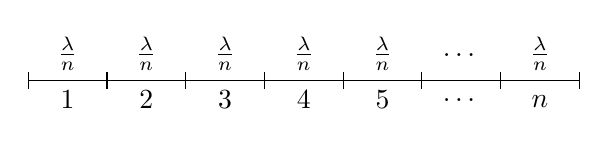
\begin{tikzpicture}

            \draw[-] (0,0) -- (7,0);
            \foreach \x in {0,1,...,7}
            \draw (\x cm,3pt) -- (\x cm,-3pt);

            \uncover<2->{
                \foreach \x in {1,2,...,5}
                \node[below] at (\x - 0.5, 0) {$\x$};
                \node[below=3pt] at (5.5, 0) {$\dots$};
                \node[below=2pt] at (6.5, 0) {$n$};
            }

            \uncover<3->{
                \foreach \x in {0,1,...,4,6}
                \node[above] at (\x + 0.5, 0) {$\frac{\lambda}{n}$};
                \node[above=5pt] at (5.5, 0) {$\dots$};
            }

        \end{tikzpicture}
    \end{figure}

    \uncover<4->{单位时间内\textcolor{blue}{实际}提交的任务数量 $X$ 服从二项分布 $X \sim B(n, p)$ :
        $$P\left\{X=k\right\} = C_n^k \, p^k (1-p)^{n-k}$$
    }

\end{frame}

\begin{frame}{对任务提交时刻的建模}

    当观察次数 $n \rightarrow \infty$ 时,表示在单位时间内持续观察用户提交任务的过程:

    \begin{equation*}
        \begin{split}
            P\left\{X=k\right\} & = \lim_{n \rightarrow \infty} C_n^k \, p^k (1-p)^{n-k}                                                                                                                              \\
            & = \lim_{n \rightarrow \infty} \frac{n(n-1)\dots(n-(k-1))}{k!} \left(\frac{\lambda}{n}\right)^k \left(1-\frac{\lambda}{n}\right)^{n-k}                                               \\
            & = \frac{\lambda^k}{k!} \lim_{n \rightarrow \infty} \frac{n(n-1)\dots(n-(k-1))}{n^k} \left(1-\frac{\lambda}{n}\right)^{-k} \colorbox{yellow}{$\left(1-\frac{\lambda}{n}\right)^{n}$} \\
            & = \frac{\lambda^k}{k!} \colorbox{yellow}{$e^{-\lambda}$}
        \end{split}
    \end{equation*}

    \uncover<2->{此时单位时间内\textcolor{blue}{实际}提交的任务数量 $X$ 服从泊松分布 $X \sim P(\lambda)$ 。}

\end{frame}

\begin{frame}{对任务提交时刻的建模}

    记 $[0,t]$ 时间段内用户提交的任务数量为 $N(t)$ ,$(s,t]$ 时间段内用户提交的任务数量为 $N(s,t] = N(t) - N(s)$ 。

    \begin{block}{\uncover<8->{泊松过程}}
        \begin{itemize}
            \item \uncover<3->{$N(0)=0$:}\uncover<2->{初始时刻没有用户提交任务}
            \item \uncover<5->{独立增量性:}\uncover<4->{在互不相交的时间段内,用户提交任务的数量相互独立}
            \item \uncover<7->{平稳增量性:}\uncover<6->{在长度相等的时间段 $t$ 内,任务提交数量服从相同的概率分布 $P(\lambda t)$}
        \end{itemize}
    \end{block}

    \uncover<9->{
        因此 $\forall s, N(s,s+t] \sim P(\lambda t)$ :
        $$P\left\{N(s,s+t]=k\right\} = \frac{(\lambda t)^k}{k!} e^{-\lambda t}$$
    }

\end{frame}

\begin{frame}{对任务提交时刻的建模}

    设 $W_n$ 为第 $n$ 个任务提交的时刻
    \uncover<2->{,$T_n$ 为第 $n-1$ 个任务与第 $n$ 个任务提交的时间间隔}
    \uncover<3->{,则 $W_n = \sum_{i=1}^{n} T_i$ 。}

    \begin{figure}
        \centering

        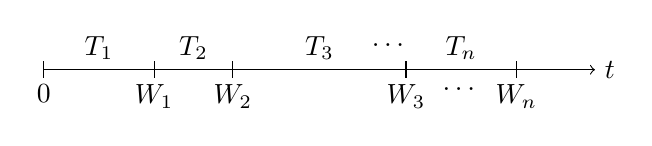
\begin{tikzpicture}
            \draw[->] (0,0) node[below=2pt] {$0$} -- (7,0) node[right] {$t$};
            \foreach \x in {0,1.4,2.4,4.6,6.0}
            \draw (\x cm,3pt) -- (\x cm,-3pt);

            \node[below=2pt] at (1.4,0) {$W_1$};
            \node[below=2pt] at (2.4,0) {$W_2$};
            \node[below=2pt] at (4.6,0) {$W_3$};
            \node[below=2pt] at (6.0,0) {$W_n$};
            \node[below=3pt] at (5.3,0) {$\dots$};

            \uncover<2->{
                \node[above] at (0.7,0) {$T_1$};
                \node[above] at (1.9,0) {$T_2$};
                \node[above] at (3.5,0) {$T_3$};
                \node[above] at (5.3,0) {$T_n$};
                \node[above=5pt] at (4.4,0) {$\dots$};
            }
        \end{tikzpicture}
    \end{figure}

    \uncover<4->{为了得到用户提交任务的时刻 $T_{submit}$ ,只需要明确 $T_n$ 服从的分布。}

\end{frame}

\begin{frame}[shrink=5]{$T_n$ 服从的分布}{$T_1$ 服从的分布}

    求 $T_1$ 的分布函数:
    \begin{align*}
         & F_{T_1}(t) = P\left\{T_1 \leqslant t\right\} = 1 - P\left\{T_1 > t\right\} = 1 - P\left\{N(0,t]=0\right\} = 1 - e^{-\lambda t} \\
         & f_{T_1}(t) = F_{T_1}'(t) = \lambda e^{-\lambda t}
    \end{align*}

    \begin{figure}
        \centering

        \begin{subfigure}[c]{0.4\textwidth}
            \begin{tikzpicture}
                \draw[->] (0,0) node[below] {$0$} -- (5,0) node[right] {$t$};
                \draw[-] (2.5,3pt) -- (2.5,-3pt) node[below] {$W_1$};
                \node[above] at (1.25,7pt) {$T_1$};
                \draw[<->] (0,5pt) -- (2.5,5pt);
                \draw[-] (3,3pt) -- (3,-3pt) node[below] {$t$};
            \end{tikzpicture}

            \caption{$T_1 \leqslant t$}
        \end{subfigure}
        \qquad
        \begin{subfigure}[c]{0.4\textwidth}
            \begin{tikzpicture}
                \draw[->] (0,0) node[below] {$0$} -- (5,0) node[right] {$t$};
                \draw[-] (2.5,3pt) -- (2.5,-3pt) node[below] {$W_1$};
                \node[above] at (1.25,7pt) {$T_1$};
                \draw[<->] (0,5pt) -- (2.5,5pt);
                \draw[-] (2,3pt) -- (2,-3pt) node[below] {$t$};
            \end{tikzpicture}

            \caption{$T_1 > t$}
        \end{subfigure}
    \end{figure}

    \uncover<2->{$T_1$ 服从指数分布:$T_1 \sim E(\lambda)$ 。}
\end{frame}

\begin{frame}[shrink=5]{$T_n$ 服从的分布}{$T_2$ 服从的分布}

    求 $T_2$ 的分布函数(假设在任意的 $s$ 时刻,第一个任务已经提交):
    \begin{equation*}
        \begin{split}
            F_{T_2}(t) &= P\left\{T_2 \leqslant t\right\} = 1 - P\left\{T_2 > t\right\} \\
            &= 1 - P\left\{N(s,s+t]=0|N(0,s]=1\right\} \\
            &= 1 - P\left\{N(s,s+t]=0\right\} \quad \text{\tiny $(0,s]$与$(s,s+t]$两时间段互不相交,相互独立} \\
            &= 1 - e^{-\lambda t}
        \end{split}
    \end{equation*}

    \begin{figure}
        \centering

        \begin{subfigure}[c]{0.4\textwidth}
            \begin{tikzpicture}
                \draw[->] (0,0) node[below] {$0$} -- (5,0) node[right] {$t$};

                \draw[-] (1,3pt) -- (1,-3pt) node[below] {$W_1$};
                \draw[-] (3.5,3pt) -- (3.5,-3pt) node[below] {$W_2$};

                \node[above] at (2.25,7pt) {$T_2$};
                \draw[<->] (1,5pt) -- (3.5,5pt);

                \node[below=1.5em] at (1,0) {$s$};
                \draw[dashed] (4,0) -- (4,-1.5em) node[below] {$s+t$};
            \end{tikzpicture}

            \caption{$T_2 \leqslant t$}
        \end{subfigure}
        \qquad
        \begin{subfigure}[c]{0.4\textwidth}
            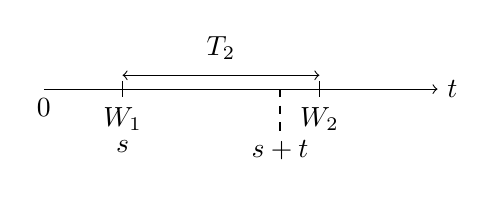
\begin{tikzpicture}
                \draw[->] (0,0) node[below] {$0$} -- (5,0) node[right] {$t$};

                \draw[-] (1,3pt) -- (1,-3pt) node[below] {$W_1$};
                \draw[-] (3.5,3pt) -- (3.5,-3pt) node[below] {$W_2$};

                \node[above] at (2.25,7pt) {$T_2$};
                \draw[<->] (1,5pt) -- (3.5,5pt);

                \node[below=1.5em] at (1,0) {$s$};
                \draw[dashed] (3,0) -- (3,-1.5em) node[below] {$s+t$};
            \end{tikzpicture}

            \caption{$T_2 > t$}
        \end{subfigure}
    \end{figure}

    \uncover<2->{根据无记忆性,$T_2,\dots,T_n$ 均服从参数为 $\lambda$ 的指数分布。}
\end{frame}

\begin{frame}[fragile]{任务提交时间序列和总计算量}

    因为 $T_n \sim E(\lambda)$ ,所以代码中对参数为 $\lambda$ 的指数分布进行采样即可得到任务提交的时间间隔。
    将时间间隔累加,即可得到任务提交的时间序列,对应 $T_{submit}$ 。

    \scriptsize
    \begin{minted}{python3}
        # 生成时间间隔
        intervalT = stats.expon.rvs(scale=1 / lamda, size=self.jobNum)
        # 对时间间隔累加得到提交时间
        self.arrival_Times = np.around(intervalT.cumsum(), decimals=3)
    \end{minted}

    \normalsize
    总计算量 $reqCom$ 通过正态分布采样。

    \scriptsize
    \begin{minted}{python3}
        self.jobsMI = np.random.normal(self.jobMI, self.jobMI_std, self.jobNum)
        self.jobsMI = self.jobsMI.astype(int)
    \end{minted}
\end{frame}

\subsection{虚拟机模型}

\begin{frame}{虚拟机属性}

    每个虚拟机具有如下属性:

    \begin{itemize}
        \item $vID$:虚拟机编号
        \item $vCom$:单核计算速度
        \item $vAcc$:多核加速系数
        \item $T_{idle}$:虚拟机处理完最后一个任务的时刻
        \item $vType$:虚拟机类型
              \begin{itemize}
                  \item 高性能计算
                  \item 高性能I/O
              \end{itemize}
        \item $vSC$:虚拟机启动开销
        \item $vEC$:虚拟机运行开销
    \end{itemize}
\end{frame}

\subsection{任务在虚拟机中的运行过程}

\begin{frame}[shrink=2]{任务在虚拟机中的运行过程}

    当一个任务在 $T_{submit}$ 时刻提交给一个虚拟机时,可以得到该任务的等待时间:
    $$T_{wait} = \max\{T_{idle} - T_{submit}, 0\}$$

    \begin{figure}
        \centering

        \begin{subfigure}[c]{0.4\textwidth}
            \begin{tikzpicture}
                \draw[->] (0,0) -- (5,0) node[right] {$t$};

                \draw[-] (0,3pt) -- (0,-3pt);
                \draw[-] (1,3pt) -- (1,-3pt) node[below] {$T_{submit}$};
                \draw[-] (4,3pt) -- (4,-3pt) node[below] {$T_{idle}$};

                \node[above] at (2.5,7pt) {需要等待的时间};
                \draw[->] (1,5pt) -- (4,5pt);
            \end{tikzpicture}

            \caption{$T_{idle} > T_{submit}$}
        \end{subfigure}
        \qquad
        \begin{subfigure}[c]{0.4\textwidth}
            \begin{tikzpicture}
                \draw[->] (0,0) -- (5,0) node[right] {$t$};

                \draw[-] (0,3pt) -- (0,-3pt);
                \draw[-] (1,3pt) -- (1,-3pt) node[below] {$T_{idle}$};
                \draw[-] (4,3pt) -- (4,-3pt) node[below] {$T_{submit}$};

                \node[above] at (2.5,7pt) {无需等待直接处理任务};
                \draw[<-] (1,5pt) -- (4,5pt);
            \end{tikzpicture}

            \caption{$T_{idle} \leqslant T_{submit}$}
        \end{subfigure}
    \end{figure}

    \uncover<2->{
        当虚拟机开始执行任务时,任务的执行时间:
        $$T_{exe} = \frac{Type \oplus vType + 1}{2} \cdot \frac{reqCom}{vCom \cdot vAcc}$$
    }
\end{frame}

\begin{frame}{运行结果指标}
    \begin{itemize}
        \item 任务响应时间:$T_{rep} = T_{wait} + T_{exe}$
        \item 是否满足 $QoS$ 要求:$success = \begin{cases}
                      1, & T_{rep} \leqslant QoS \\ 0,& \text{otherwise}
                  \end{cases}$
        \item 虚拟机费用:$cost = vSC + vEC \cdot T_{exe}$
    \end{itemize}
\end{frame}


\section{Deep Q-Learning}

\input{src/DQN.tex}

\section{Baseline}

\begin{frame}{作为Baseline的3种算法}

    \begin{itemize}
        \item Random:将任务随机分配给任意一台虚拟机
        \item Round-Robin:将任务轮流分配给每台虚拟机
        \item Earliest:将任务分配给最先完成任务(即 $T_{idle}$ 最小)的虚拟机
    \end{itemize}

\end{frame}


\setbeamertemplate{sidebar left}{}

\begin{frame}

    \centering
    \Huge
    \usefont{OT1}{pzc}{m}{n}
    Fin.

\end{frame}

\end{document}
